\documentclass[a4paper,10pt]{article}
\usepackage{graphicx} % Required for inserting images
\usepackage[nswissgerman]{babel}
%4 stackanchor  
\usepackage{stackengine}
% define nice looking boxes
\usepackage[many]{tcolorbox}

% a base set, that is then customised
\tcbset {
  base/.style={
    boxrule=0mm,
    leftrule=1mm,
    left=1.75mm,
    arc=0mm, 
    fonttitle=\bfseries, 
    colbacktitle=black!10!white, 
    coltitle=black, 
    toptitle=0.75mm, 
    bottomtitle=0.25mm,
    title={#1}
  }
}
\definecolor{brandblue}{rgb}{0.34, 0.7, 1}
\newtcolorbox{mainbox}[1]{
  colframe=brandblue, 
  base={#1}
}

\definecolor{orange}{rgb}{1, 0.55, 0.3}
\newtcolorbox{tbox}[1]{
  colframe=orange, 
  base={#1}
}

\definecolor{green}{rgb}{0.294, 0.729, 0.254}
\newtcolorbox{bembox}[1]{
  colframe=green, 
  base={#1}
}

\definecolor{red}{rgb}{0.99, 0.04, 0.99}
\newtcolorbox{tipbox}[1]{
  colframe=red, 
  base={#1}
}

\newtcolorbox{defbox}[1]{
  colframe=black!20!white,
  base={#1}
}
% Mathematical typesetting & symbols
\usepackage{amsthm, mathtools, amssymb} 
\usepackage{marvosym, wasysym}


\allowdisplaybreaks

% Tables
\usepackage{tabularx, multirow}
\usepackage{booktabs}
\renewcommand*{\arraystretch}{2}

% Make enumerations more compact
\usepackage{enumitem}
\setitemize{itemsep=0.5pt}
\setenumerate{itemsep=0.75pt}

% To include sketches & PDFs
\usepackage{graphicx}

% For hyperlinks
\usepackage{hyperref}
\hypersetup{
  colorlinks=true
}
% Math helper stuff
\def\limn{\lim_{n\to \infty}}
\def\limxo{\lim_{x\to 0}}
\def\limxi{\lim_{x\to\infty}}
\def\limxn{\lim_{x\to-\infty}}
\def\sumk{\sum_{k=1}^\infty}
\def\sumn{\sum_{n=0}^\infty}
\def\R{\mathbb{R}}
\def\dx{\text{ d}x}
\usepackage[utf8]{inputenc}

\title{Vorlesung}
\author{Konstantin Lucny}
\date{HS 2023}

\begin{document}
\maketitle
\section{Vorlesung}
\subsection{Structure of C++}
\begin{itemize}
    \item You \textbf{must} declare functions before they are called from a different function (no forward declarations); with the declaration you declare the compiler the return types and input types
    \item int main() is the only \textbf{non-void} method that does \textbf{not} need a return statement  
\end{itemize}
\subsection{Similarities between Java and C++}
\begin{itemize}
    \item Case sensitivity, curly braces, parentheses, semicolon, comments
    \item $+,*,=,+=,==,++,<,\&\&,...$
    \item Fundamental types: \textit{int, float, double, char, bool}; also void
    \item Control structures: return, if-else, switch, for, while, ....
    \item Code modularity: Functions, classes; Namespaces
\end{itemize}
\subsection{Differences: Fundamental Types in C++}
\begin{itemize}
    \item Signed and \textbf{unsigned} integral types (int vs. unsigned int [or just unsigned])
    \item Width of \textit{bol, char, int, long} is \textbf{implementation defined}, with lower bounds (E.g. an \textit{int} is at least 16 bits wide, a \textit{long} 32 bit)
\end{itemize}
\subsection{Behavior in C++}
\begin{itemize}
    \item \textbf{Implementation-defined behaviour}: behaviour may vary, must be documented
    \item \textbf{Unspecified behaviour}: implementation-defined, no need to document
    \item \textbf{Undefined behaviour}: if present, program is not required to do anything meaningful
\end{itemize}
\subsection{Common Sources of Undefined Behaviour}
\begin{itemize}
    \item \textit{Signed} integer over-/underflow (Java: well-defined)
    \item Out of bounds array access (e.g. \textit{data[data.size()]}); C++: \textit{data.at(idx)} performs runtime check
    \item Null-pointer dereferencing
    \item Read \& write same memory location in single expression, e.g. \textit{cout << (x + x++)}
    \item Reading uninitialized variables
    \item Accessing destructed objects/deallocated memory
\end{itemize}
\subsection{Undefined Behaviour}
\begin{itemize}
    \item Compile- or runtime checks might be performed, but no guarantees
\end{itemize}
\subsection{Java vs. C++ Differences: Initialisation}
\begin{itemize}
    \item C++ default-initialises variables iff the type declares a default constructor
    \item No default constructors for fundamental types (int, double, ...)
    \begin{figure}[htp]
        \centering
        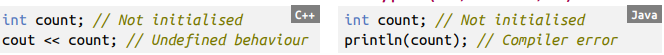
\includegraphics[width=15cm]{e1.png}
        \caption{Constructur C++}
        \label{fig:enter-label}
    \end{figure}
    \item C++: reading uninitialised variables is undefined behaviour
\end{itemize}
\subsection{Differences: Type Inference}
\begin{itemize}
    \item C++ is statically typed, just like Java
    \item Limited support for type inference includes keyword \textit{auto} and Type parameter interference → templates, 2nd week
    \item Def. \textit{auto}: C++ tries to figure out which type the variable should be
    \begin{figure}[htp]
        \centering
        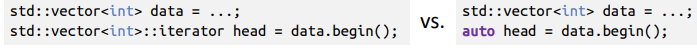
\includegraphics[width=15cm]{e2.png}
        \caption{Caption}
        \label{fig:enter-label}
    \end{figure}
    \item Types serve as code documentation → don’t overuse \textit{auto}
\end{itemize}
\subsection{Values vs. References}
\textbf{Important}: C++ always copies what is put in a function \textbf{unless} it is specificly mentioned to take the reference/pointer/etc...\\
\begin{itemize}
    \item By default, types in C++ are value types (in Java primitive types)
    \item Value types (of statically-known size) can be allocated on the stack
    \item Pass by value: values are copied upon function calls
    \item Return by value: analogous
\end{itemize}
\subsection{Values vs. Pointers}
\begin{itemize}
    \item Java’s references are (a simplified version of) pointers in C++
    \begin{figure}[htp]
        \centering
        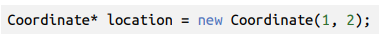
\includegraphics[width=10cm]{e3.png}
        \caption{Pointer C++}
        \label{fig:enter-label}
    \end{figure}
    \item C++ has no garbage collector → manual memory management (every \textit{new} needs a \textit{delete}
    \item Pointers are not relevant for NumCS → not discussed further
\end{itemize}
\subsection{Pass by Reference / Reference Types}
Values can be shared via \textit{C++ references} (use a \& after type declaration; e.g. \textit{void swap(Coordinate\& c)})
\begin{figure}[htp]
    \centering
    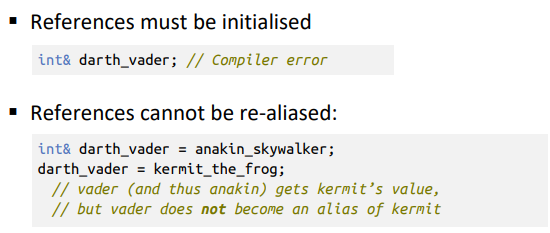
\includegraphics[width=12cm]{e4.png}
    \caption{Refernces Info}
    \label{fig:enter-label}
\end{figure}
\subsection{Constant variables}
Java's \textit{final} is \textit{const} in C++ (compiler error when trying to change \textbf{const} variable\\
A program is \textbf{const-correct} if all variables not intended to be mutated are typed as \textit{const}
\subsection{Overloading}
In contrast to Java, C++ \textbf{supports} overloading of operators
\begin{figure}[htp]
    \centering
    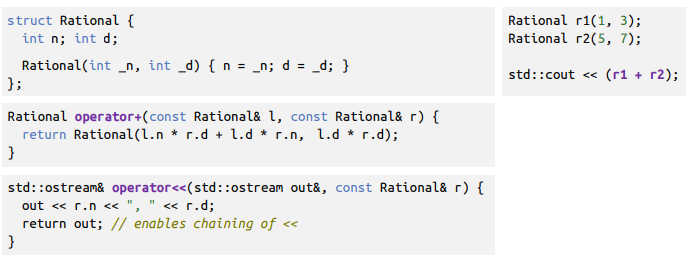
\includegraphics[width=15cm]{e5.png}
    \caption{Overloading operators}
    \label{fig:enter-label}
\end{figure}
\subsection{Semantics of \textit{\#include} vs. Separate Compilation}
\begin{figure}[htp]
    \centering
    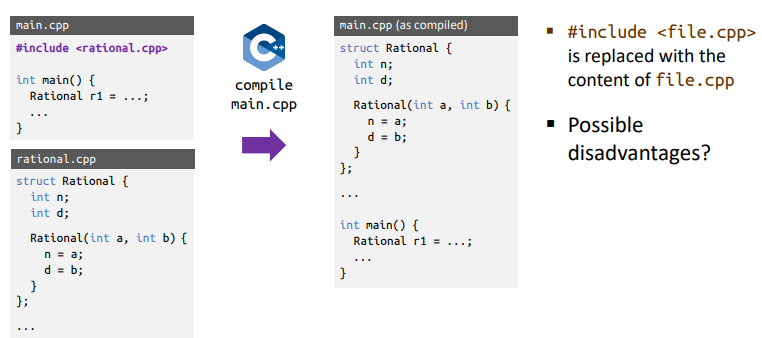
\includegraphics[width=15cm]{e6.png}
    \caption{Semantics of \#include}
    \label{fig:enter-label}
\end{figure}
\textbf{Fact}: \#include <lib.cpp> is replaced with the contents of file lib.cpp\\
New goal: Enable \textbf{separate} compilation of units of code (e.g. classes, libraries); resulting machine code then linked afterwards.\\
\textbf{C++ solution}:  Separation of declarations from definitions in separate files (Header files \textit{.h} contain declarations, implementations reside in .cpp files)
\begin{figure}[htp]
    \centering
    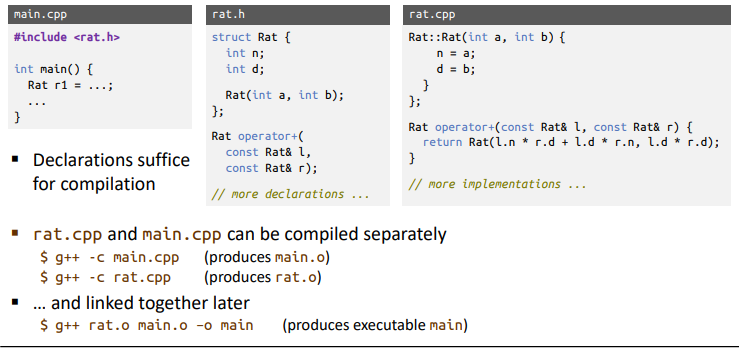
\includegraphics[width=16cm]{e7.png}
    \caption{.h Files}
    \label{fig:enter-label}
\end{figure}
\section{Lecture (\today)}
\subsection{Classes}
\begin{figure}[h]
    \centering
    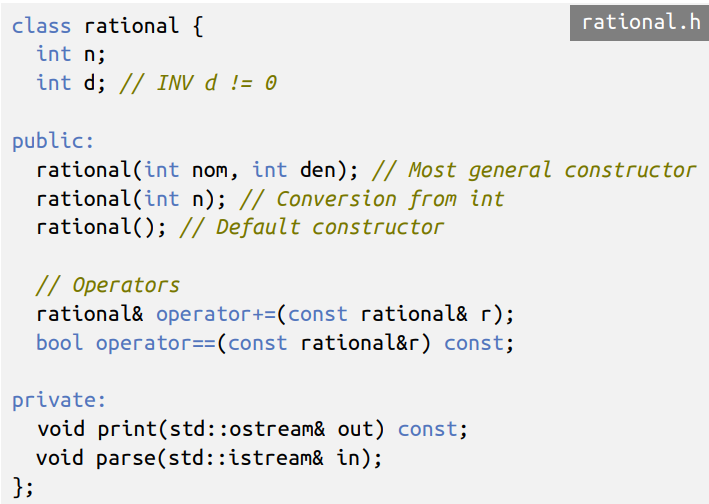
\includegraphics[width=0.7\linewidth]{e8.png}
    \caption{Example class in C}
    \label{fig:enter-label}
\end{figure}
\begin{figure}
    \centering
    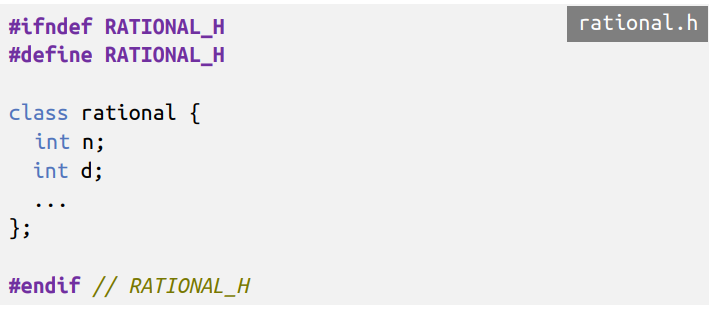
\includegraphics[width=0.75\linewidth]{e9.png}
    \caption{Header file example}
    \label{fig:enter-label}
\end{figure}
\begin{tipbox}
    {Important}
    include guards (violet code in example above; more information in Lecture 1)
\end{tipbox}
\begin{tbox}
    {Struct vs. class}
    \textit{class} members are private by default, \textit{struct} members are public by default
\end{tbox}
\begin{itemize}
    \item Usually structs hold data, provide little functionality
    \item Classes for functionality
\end{itemize}
\begin{tbox}
    {Keyword \textit{this}}
    \textit{this} is a pointer; hence you have to dereference it \textit{(*this)} to access its data/variables...
\end{tbox}
\subsubsection{Member Variable}
    Use initialiser lists (left), not assignments (reason: performance)
    \begin{figure}[h]
        \centering
        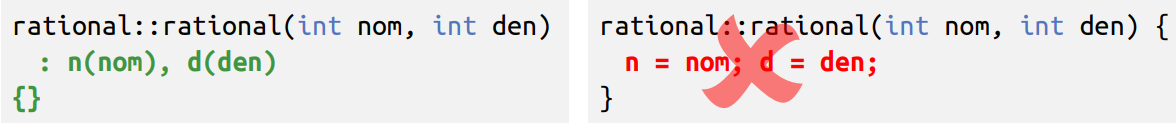
\includegraphics[width=1\linewidth]{e10.png}
        \caption{initializer lists(left); right one also works}
        \label{fig:enter-label}
    \end{figure}

\pagebreak
\subsubsection{Constructors}
\begin{figure}[h]
    \centering
    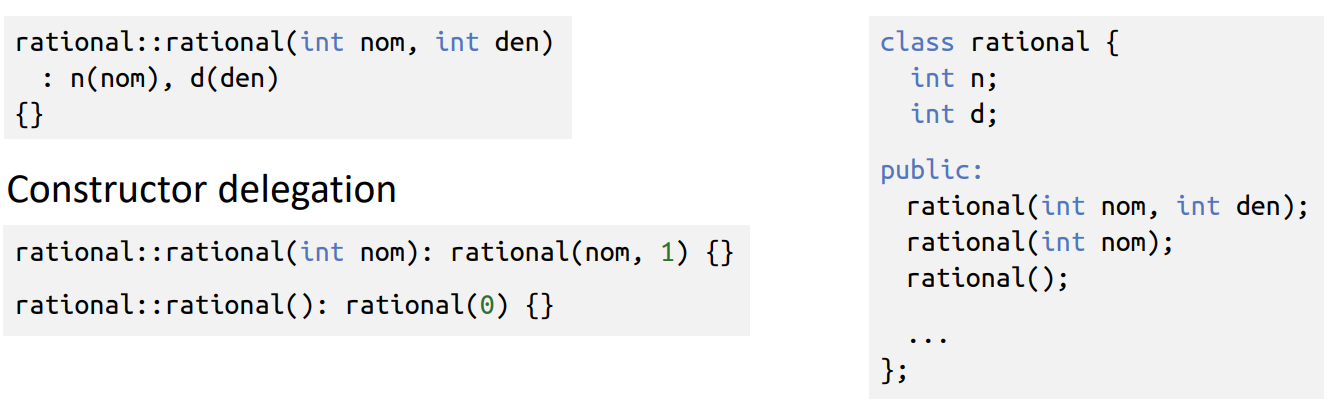
\includegraphics[width=1\linewidth]{e12.png}
    \caption{Example of Constructors calling constructors}
    \label{fig:enter-label}
\end{figure}
Constructors can call other constructors (converting constructors)
\begin{figure}[h]
    \centering
    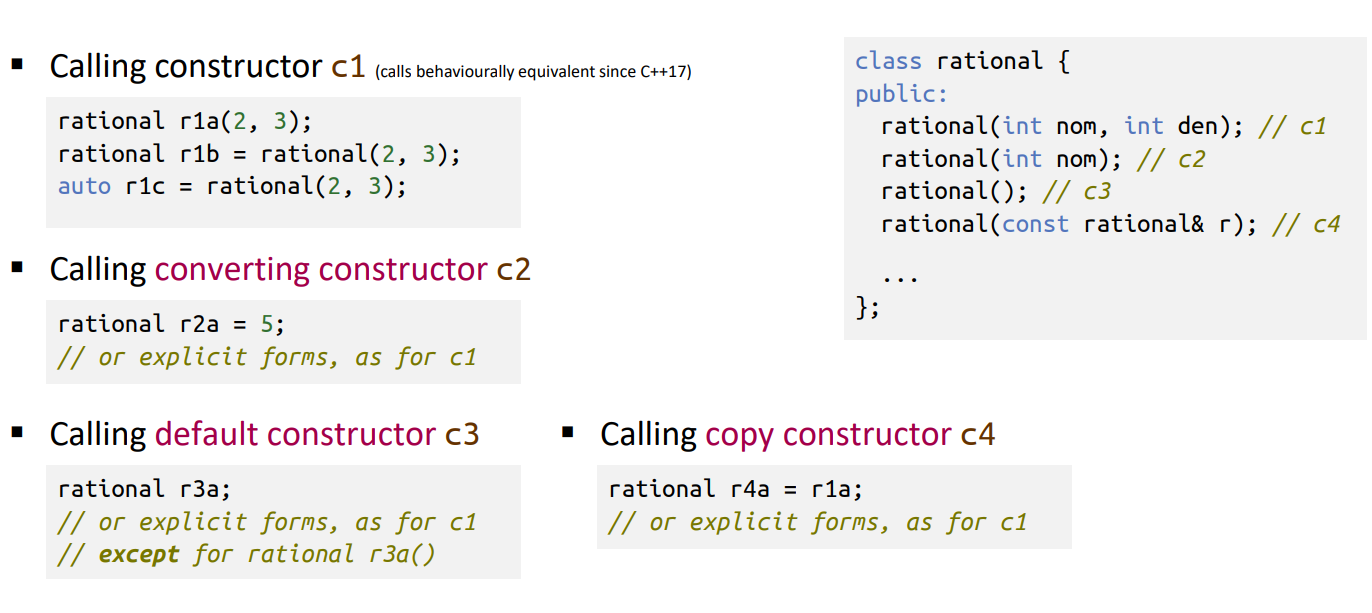
\includegraphics[width=1\linewidth]{e11.png}
    \caption{Constructor call-sites}
    \label{fig:enter-label}
\end{figure}

\pagebreak
\subsection{Initialisation vs. Assignments}
\begin{figure}[h!]
    \centering
    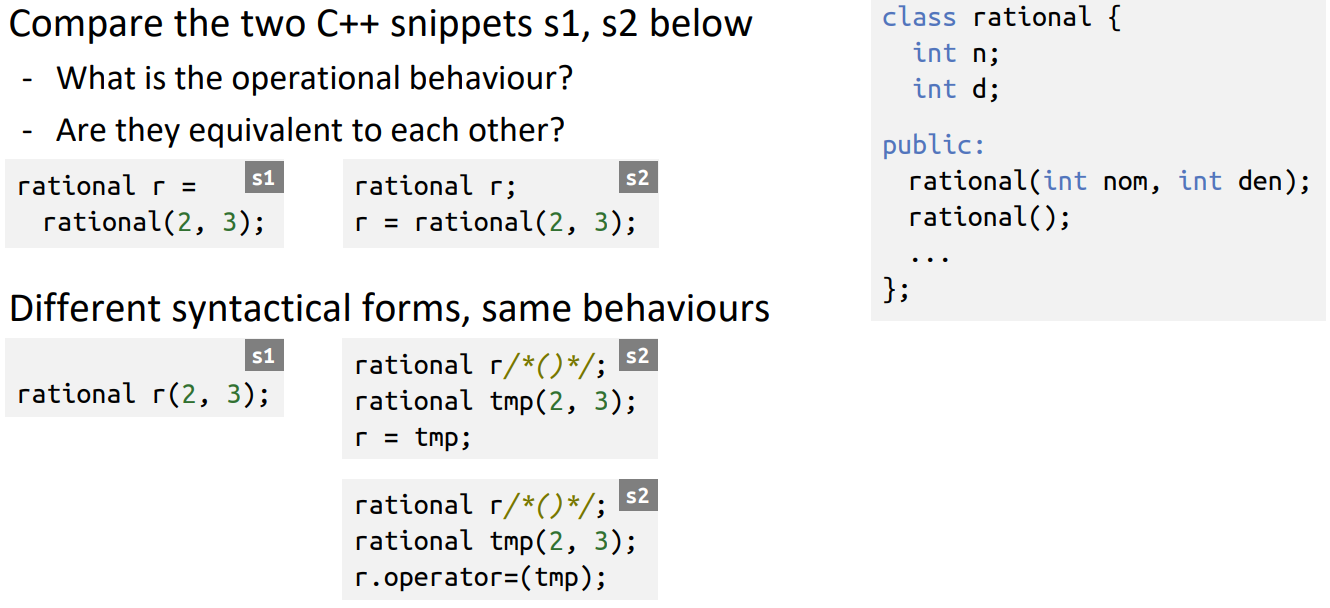
\includegraphics[width=1\linewidth]{e13.png}
    \caption{Example Initialization vs. Assignment}
    \label{fig:enter-label}
\end{figure}
\textbf{Description} of example above: For s2 \textit{r} is really a value (\textbf{not} a reference) hence when we construct \textit{rational(2, 3)} we really change the value of \textit{r} and \textbf{not} the reference.
\begin{tipbox}
    {Compiler Generated member functions}
    \textbf{copy constructor} creates new object 
    \\\textbf{assignment constructor} just overwrites object
\end{tipbox}
\subsection{\textit{Const} Member Functions}
\begin{figure}[h]
    \centering
    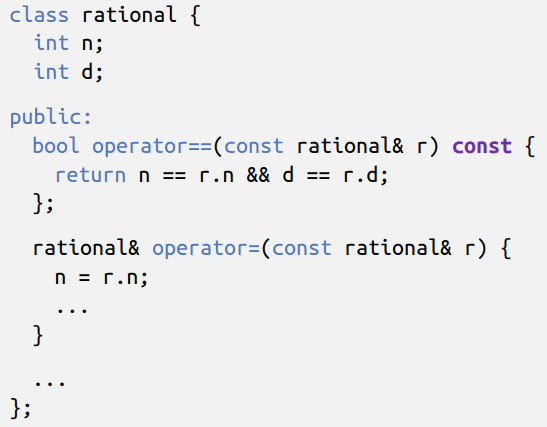
\includegraphics[width=0.7\linewidth]{e14.png}
    \caption{const member function}
    \label{fig:enter-label}
\end{figure}
\begin{itemize}
    \item Equality operator is const
    \begin{itemize}
        \item Cannot modify receiver’s member
        variables (this->n/d)
        \item stronger guarantee to callers
    \end{itemize}
    \item Assignment operator \textbf{cannot} be \textit{const}
    \item Only \textit{const} member functions can be invoked on a \textit{const} receiver
\end{itemize}
\subsection{Object Lifetimes and References}
\subsubsection{Static Memory: Scope-Based Lifetimes}
\begin{itemize}
    \item Statically allocated objects have scope-based lifetimes (in C++)
    \item Compiler can insert deallocation code to automatically destroy object at scope end
\end{itemize}
Objects are destroyed at scope end → problem with references? Yes could be an issue. Hence, it is your own responsibility that objects stay in scope longer than any reference to them.
\begin{bembox}
    {Why return by reference?}
    \begin{itemize}
        \item Give callers access to values inside other values (e.g. container, object graphs)
    \end{itemize}
\end{bembox}
 \begin{figure}[h]
            \centering
            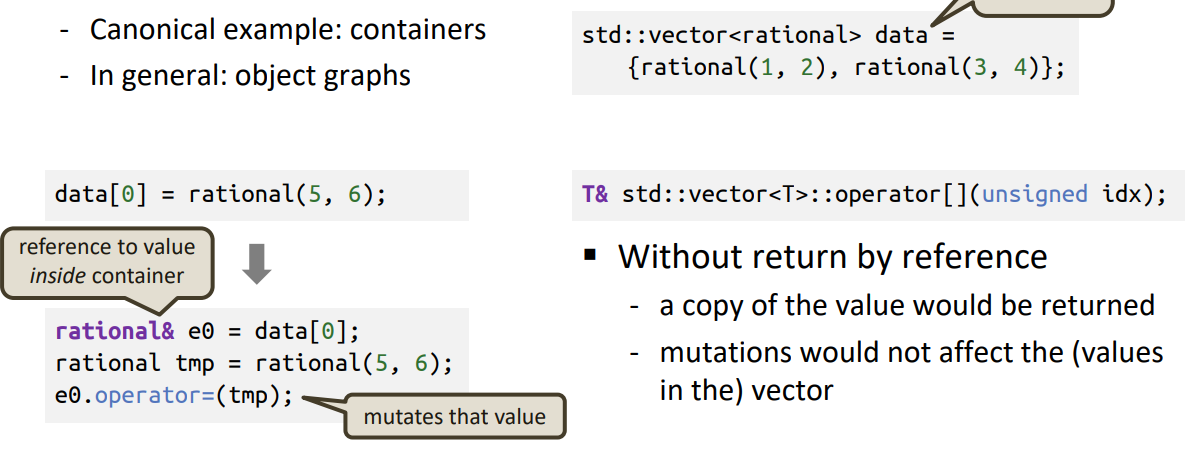
\includegraphics[width=0.75\linewidth]{e15.png}
            \caption{Example container return by reference}
            \label{fig:enter-label}
        \end{figure}
\pagebreak
\subsection{C++ containers}
\begin{figure}[h!]
    \centering
    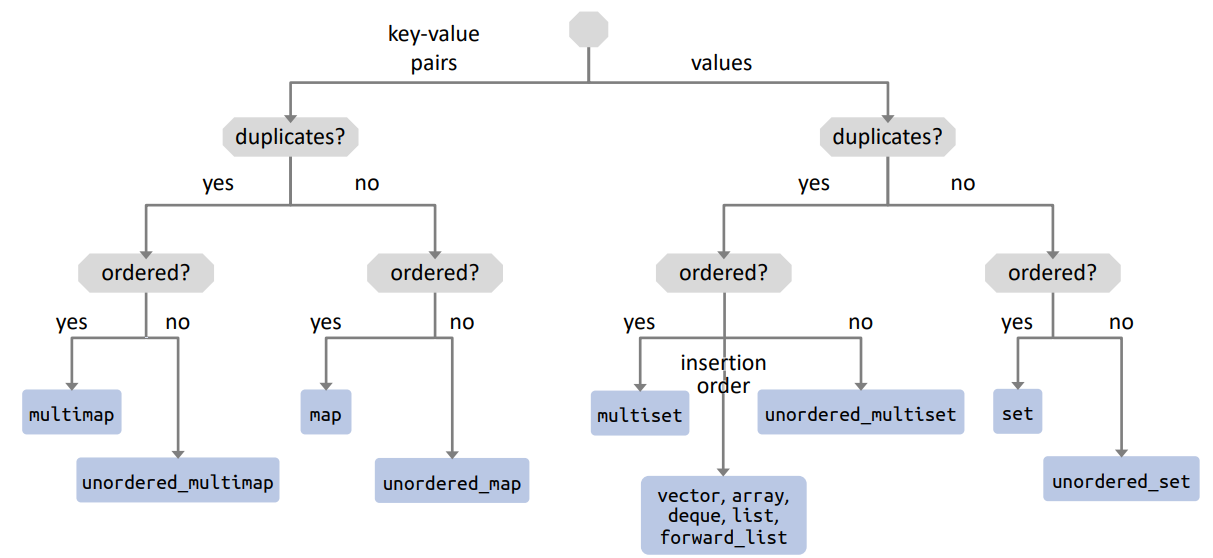
\includegraphics[width=1\linewidth]{e16.png}
    \caption{overview C++ containers (like Java collections)}
    \label{fig:enter-label}
\end{figure}
\subsection{Iterators}
\begin{figure}[h!]
    \centering
    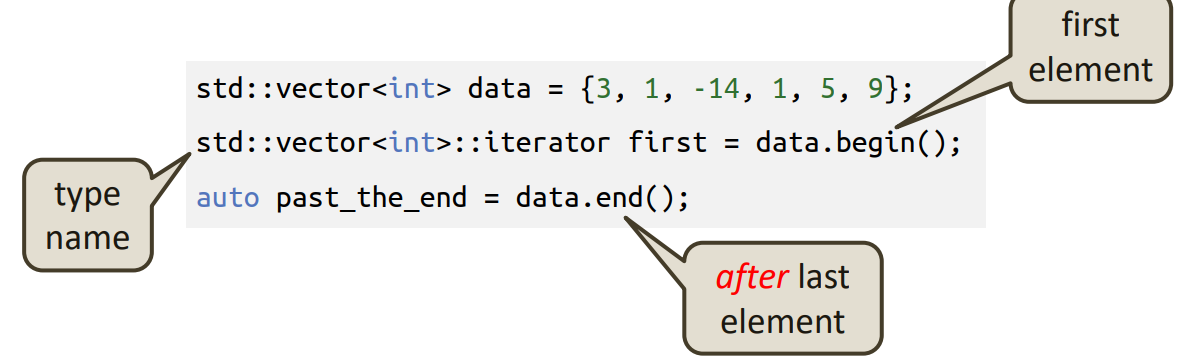
\includegraphics[width=1\linewidth]{e17.png}
    \caption{Iterator example}
    \label{fig:enter-label}
\end{figure}
\begin{figure}[h!]
    \centering
    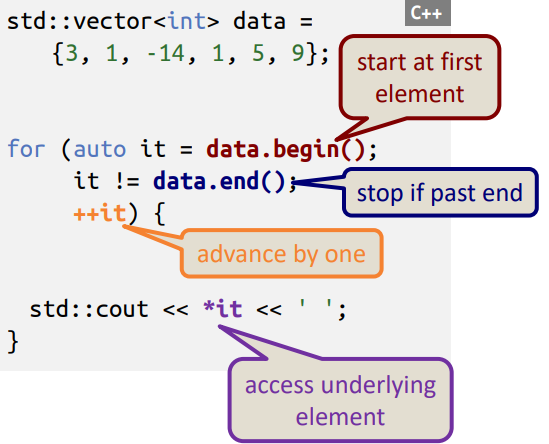
\includegraphics[width=1\linewidth]{e18.png}
    \caption{\textbf{Example}: Iterator in for loop}
    \label{fig:enter-label}
\end{figure}
\subsubsection{Interlude: Range-Based for-Loop}
\begin{figure}[h]
    \centering
    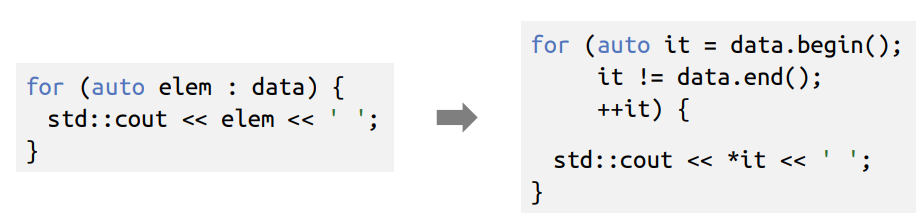
\includegraphics[width=1\linewidth]{e19.png}
    \caption{Compiler desugares range-based for-loop into iterator-based loop}
    \label{fig:enter-label}
\end{figure}
\subsection{Eigen}
\begin{figure}[h]
    \centering
    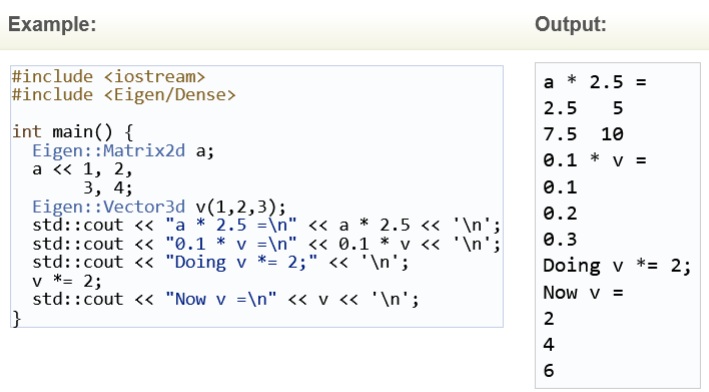
\includegraphics[width=1\linewidth]{e20.png}
    \caption{Enter Caption}
    \label{fig:enter-label}
\end{figure}
\begin{figure}
    \centering
    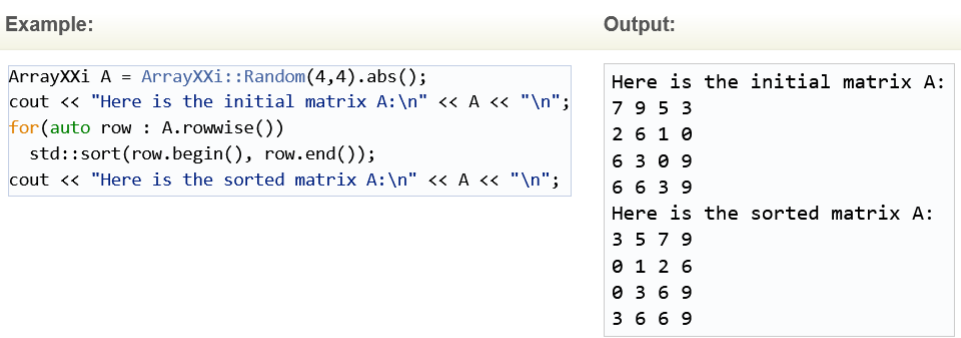
\includegraphics[width=1\linewidth]{e21.png}
    \caption{Enter Caption}
    \label{fig:enter-label}
\end{figure}
\end{document}
